\documentclass[twoside]{article}
\newcommand{\magic}{}
\usepackage{klsh24-styles}

\begin{document}

\thispagestyle{empty}
\import{./}{titlepage.tex} 

\thispagestyle{empty}
\import{./}{photopage.tex} 
\newpage

\thispagestyle{empty}
\import{./}{abstract.tex}
\begin{figure}[h]
    \centering
    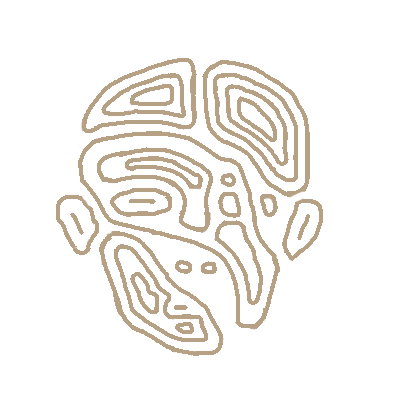
\includegraphics[width=0.7\textwidth]{chelik.png}
    \label{fig:abstract}
\end{figure}
\vfill
\pagebreak

\setcounter{page}{1}
\tableofcontents
\pagebreak

\section{Счет углов}
\epigraph{скажи им, что нужно быть счастливыми и что главное стать хорошим человеком}{дед всегда прав}

\import{sections/}{counting_angles.tex}

\subsection*{Задачи}
\addcontentsline{toc}{subsection}{Задачи}
Было тяжело подобрать задачи, в которых требуется исключительно доказательство перпендикулярности; поэтому тут задачи, которые в целом хорошо делаются счетом углов, а не только на ортогональность.

\import{tasks/}{counting_angles.tex}

\section{Свойства ортоцентра}
{\begin{minipage}{0.55\linewidth}
    \begin{definition}\label{def:orthocenter}
        Ортоцентр \textbf{H} -- это точка пересечения высот треугольника.
    \end{definition}
    Я всегда буду ортоцентр треугольника $ABC$ обозначать {\color{OliveGreen}\textbf{большой зеленой точкой}} \textit{(просто я так решил)}, а центр описанной окружности как выколотую \textit{(так уже более принято)}.
\end{minipage}
\hfill
\begin{minipage}{0.4\linewidth}
    \begin{asy}
        size(4.8cm);
        triangle t = triangle((point)(0, 3.7), (point)(-1.5, 0), (point)(3, 0));
        draw(t, linewidth(bp));
        point H = orthocentercenter(t);

        draw(segment(t.VA, foot(t.VA)), grey); perpendicularmark(t.BC, line(t.VA, foot(t.VA)), blue, size=7);
        draw(segment(t.VB, foot(t.VB)), grey); perpendicularmark(t.AC, line(t.VB, foot(t.VB)), blue, quarter=3, size=7);
        draw(segment(t.VC, foot(t.VC)), grey); perpendicularmark(t.AB, line(t.VC, foot(t.VC)), blue, size=7);
        
        dot("$H$", H, 1.2N + .7E, hpen);
        dot("$O$", circumcenter(t), SE, filltype=FillDraw(fillpen=white, drawpen=black));
    \end{asy}
\end{minipage}}

\subsection{Симметрии ортоцентра}
\import{sections/}{symmetry_orthocenter.tex}

\subsection{Остальные свойства ортоцентра}
\import{sections/}{other_orthocenter.tex}

\subsection{Окружность Эйлера}
\import{sections/}{euler_circle.tex}

\subsection*{Задачи}
\addcontentsline{toc}{subsection}{Задачи}
\import{tasks/}{orthocenter}

\frule{0.382}{0.618}

\import{tasks/}{euler_circle.tex}


\section{Ортодиагональные четырёхугольники}
\import{sections/}{diagonals.tex}

\subsection*{Задачи}
\addcontentsline{toc}{subsection}{Задачи}
\import{tasks/}{diagonals.tex}


\section{Радикальная ось и линия центров}
Не всегда удается "счетом углов" доказать принадлежность четверки точек одной окружности. Часто нужно использовать "счет в отрезках". С этим нам помогает степень точки. А чтобы доказать, что три прямые пересекаются в одной точке, можно сказать что это радикальный центр какой-то тройки окружностей.
\subsection{Степень точки}
\import{sections/}{pow.tex}

\subsection{Радикальная ось}
\import{sections/}{radical.tex}

\subsection*{Задачи}
\addcontentsline{toc}{subsection}{Задачи}
\epigraph{Судя по карте, дорога здесь одна.

Трясет на ухабах — мы переносим с одобреньем.}{Александр Башлачёв}
\noindent Простите меня заранее за такие трудные задачи. Если вы отвалитесь довольно рано -- не горюйте. Я вам всегда помогу! Удачи {\color{red}{$\heartsuit$}}
\import{tasks/}{pow_radical.tex}


\section{Известные конструкции}

Этот раздел посвящен тому, чтобы при доказательстве пер\-пен\-ди\-ку\-ляр\-нос\-ти использовать какие-то известные вам конструкции (прямая Симсона, задача №255, или что вы там знаете..). Таких очень много, и это то, что по-сути и остается только изучать. Да и все, что мы до этого с вами проходили, можно тоже называть известными конструкциями.

\subsection{Прямая Симсона}
\import{sections/}{simson_line.tex}

\subsection{Задача №255}
\setlength{\epigraphwidth}{0.8\linewidth}\epigraph{Наверное, каждая содержательная геометрическая задача может быть источником целого ряда новых. Для этого с ней надо некоторое время <<повозиться>>, посмотреть с разных сторон, попробовать перефразировать, обобщить. В результате удивительным образом может возникнуть новая, совершенно не похожая на <<родителя>> задача. Например, возьмём ту же задачу №255...}{И. Ф. Шарыгин. Геометрия. Задачник 9–11}

\import{sections/}{lemma255.tex}

\subsection*{Задачи}
\addcontentsline{toc}{subsection}{Задачи}
\import{tasks/}{simson_line.tex}

\frule{0.382}{0.618}

\noindent Эта серия задач довольно простая,  потому что у нас последнее (!) занятие.  Ну и вы, кажется, должны были устать от "Симсона"\;и "cтепени точки". Поэтому отдыхайте и наслаждайтесь задачами! {\color{red}{$\heartsuit$}}
\import{tasks/}{lemma255.tex}

\appendix 

\newpage \pagenumbering{roman} 

\section{Анкета}
\sffamily \import{./}{survey.tex} \newpage

\section{Заметки}
\begin{table}[b]
    \sffamily
    \rowcolors{2}{blue!25}{red!25}
    \centering
    \begin{tabular}{|l|c|c|}
        \hline
        \textbf{Награда} & \textbf{Доля от количества} & \textbf{Количество {\large$\square$}} \\ \hline
        Конфета & $33\%$ & 14 \\ \hline
        Дошик & $50\%$ & 21 \\ \hline
        Шоколадка & $70\%$ & 29 \\ \hline
        Значок& $90\%$ & 38 \\ \hline
        \rowcolor{yellow!40} Общее количество & $100\%$ & \thewishlist \\ \hline
    \end{tabular}
    \label{tab:Ништяки}
    \caption{Таблица ништяков.}
\end{table}
\newpage
\rmfamily

\thispagestyle{empty} \import{./}{radioheadsong.tex}

\if\magic S{
\newpage \thispagestyle{empty} \import{./}{radioheadtable.tex} 

}\else{}\fi

\end{document}
